\textit{Diseñar e implementar una heurística de búsqueda local para CIDM.}

\subsection{Ejercicio A}

\textit{Explicar detalladamente el algoritmo implementado. Plantear al menos dos vecindades distintas para la búsqueda y al menos dos soluciones iniciales.}

\medskip

\subsubsection{Algoritmo implementado}

Sea G=(V,E) un grafo simple, la heurística de búsqueda local propuesta genera una solución inicial valida, es decir un V' $\subseteq$ V que es dominante e independiente (CID), de dos formas:
\begin{enumerate}
	\item \textbf{Heurística constructiva golosa}: procedimiento descripto en el ejercicio anterior.
    \item \textbf{Procedimiento BFS modificado}: detallado a continuación.

\end{enumerate}

\subsubsection{Procedimiento BFS modificado:}

Partimos de incluir un vértice inicial $v$ a $V'$ y luego vamos a ir agregando vértices a $V'$ determinando si el vértice analizado debe incluirse en $V'$.
El BFS modificado funciona de la siguiente manera:
\medskip

\begin{codesnippet}
Los vértices están numerados de 0 a n-1.

Creamos un vector, llamado solucionInicial, de tamaño n para guardar el estado de los
vértices (si fue VISITADO o no)

Creamos un vector de tamaño n en donde para cada posición guardamos si
pertenece al CID (INCLUIDO o no)

Al vértice inicial v lo ponemos como VISITADO y INCLUIDO y lo incluimos en la cola.

Luego mientras no este vacía la cola:
    Sacamos el primer elemento de la cola (w) y lo ponemos INCLUIDO.
    Revisamos cada adyacente a w:
        Si algún adyacente esta INCLUIDO entonces hacemos w = NO INCLUIDO.
        Si el adyacente no fue VISITADO entonces lo ponemos como VISITADO y
        lo agregamos a la cola.

Repetimos el procedimiento para el resto de las componentes conexas, empezando por
el vértice de menor numeración de la componente analizada.
\end{codesnippet}

A continuación mostramos un ejemplo del recorrido BFS, en donde el vértice 0 ya fue visitado y se esta analizando sus adyacentes, en particular el vértice 1, el cual es provisoriamiente INCLUIDO:
\medskip

\tikz[every node/.style={draw,circle}] {
\node[fill=blue!40, text=white] (1) at (0, 0)  { 0 };
\node[fill=red!40, text=white] (2) at (2, 0)  { 1 };
\node (5) at (4, 0)  { 3 };
\node (6) at (6, 0)  { 4 };
\node (7) at (3,-1)  { 2 };
\draw (1) edge node[above,draw=none] {} (2);
\draw (5) edge node[above,draw=none] {} (6);
\draw (2) edge node[above,draw=none] {} (7);
}

Para luego ser desmarcado debido a la presencia de un adyacente INCLUIDO, siendo la solución generada la siguiente:
\medskip

\tikz[every node/.style={draw,circle}] {
\node[fill=blue!40, text=white] (1) at (0, 0)  { 0 };
\node (2) at (2, 0)  { 1 };
\node[fill=blue!40, text=white] (5) at (4, 0)  { 3 };
\node (6) at (6, 0)  { 4 };
\node[fill=blue!40, text=white] (7) at (3,-1)  { 2 };
\draw (1) edge node[above,draw=none] {} (2);
\draw (5) edge node[above,draw=none] {} (6);
\draw (2) edge node[above,draw=none] {} (7);
}



\subsubsection{Primer Criterio de Vecindad}

El primer criterio de vecindad implementado consiste en generar soluciones vecinas a partir de quitar k vértices que pertenecen al subconjunto CID de la solución inicial y agregar 1 vértice al subconjunto, donde k $\in \mathbb{N}$ y k $\geq$ 2. Logrando de esta manera una reducción en el cardinal del subconjunto CID de, al menos, un vértice.

Para llevar adelante exitosamente este intercambio, debemos buscar aquellos vértices no incluidos en CID en la solución inicial, que tengan, al menos, dos vértices adyacentes incluidos en CID, para poder incluir ese vértice en la solución vecina y quitar sus adyacentes.

\begin{itemize}
	\item Ejemplo de un cambio 4 por 1:

    \tikz[every node/.style={draw,circle}] {
		\node[fill=blue!40, text=white] (1) at (0, 0)  { 0 };
		\node (2) at (1, -1)  { 1 };
		\node[fill=blue!40, text=white] (5) at (2, -2)  { 3 };
		\node[fill=blue!40, text=white] (7) at (2, 0)  { 2 };
		\node[fill=blue!40, text=white] (8) at (0, -2)  { 4 };
		\node (9) at (5, 0)  { 0 };
		\node[fill=blue!40, text=white] (10) at (6, -1)  { 1 };
		\node (11) at (7, -2)  { 3 };
		\node (12) at (7, 0)  { 2 };
		\node (13) at (5, -2)  { 4 };
		\draw (1) edge node[above,draw=none] {} (2);
		\draw (5) edge node[above,draw=none] {} (2);
		\draw (2) edge node[above,draw=none] {} (7);
		\draw (2) edge node[above,draw=none] {} (8);
		\draw (9) edge node[above,draw=none] {} (10);
		\draw (11) edge node[above,draw=none] {} (10);
		\draw (10) edge node[above,draw=none] {} (12);
		\draw (10) edge node[above,draw=none] {} (13);
}

\end{itemize}

Sin embargo, para lograr una solución valida, los vértices quitados no pueden tener otros vértices adyacentes no incluidos en el subconjunto que, a su vez, no sean adyacentes al vértice agregado  y no sean dominados por otro vértice.

\begin{itemize}
	\item Ejemplo de solucion invalida:

    \tikz[every node/.style={draw,circle}] {
		\node[fill=blue!40, text=white] (1) at (0, 0)  { 0 };
		\node (2) at (1, -1)  { 1 };
		\node[fill=blue!40, text=white] (5) at (2, -2)  { 3 };
		\node[fill=blue!40, text=white] (7) at (2, 0)  { 2 };
		\node[fill=blue!40, text=white] (8) at (0, -2)  { 4 };
		\node (14) at (3.5, 0)  { 5 };
		\node (9) at (5, 0)  { 0 };
		\node[fill=blue!40, text=white] (10) at (6, -1)  { 1 };
		\node (11) at (7, -2)  { 3 };
		\node (12) at (7, 0)  { 2 };
		\node (13) at (5, -2)  { 4 };
		\node (15) at (8.5, 0)  { 5 };
		\draw (1) edge node[above,draw=none] {} (2);
		\draw (5) edge node[above,draw=none] {} (2);
		\draw (2) edge node[above,draw=none] {} (7);
		\draw (2) edge node[above,draw=none] {} (8);
		\draw (7) edge node[above,draw=none] {} (14);
		\draw (9) edge node[above,draw=none] {} (10);
		\draw (11) edge node[above,draw=none] {} (10);
		\draw (10) edge node[above,draw=none] {} (12);
		\draw (10) edge node[above,draw=none] {} (13);
		\draw (12) edge node[above,draw=none] {} (15);
}

\end{itemize}

El procedimiento de búsqueda de los posibles soluciones vecinas funciona de la siguiente manera:
\medskip

\begin{codesnippet}
Para todo vertice, u, en el Grafo:
  Creamos un vector de tamaño n, llamado solucionAuxiliar, al cual le copiamos
  el contenido de la solucionInicial.
  Si solucionInicial[u] = NO INCLUIDO y |adyacentes a u| > 1 entonces:
     solucionAuxiliar[u] = INCLUIDO
     cantAdyacentesIncluidos = 0
     Para todo adyacente, v, de u:
         Si solucionInicial[v] = INCLUIDO entonces:
             cantAdyacentesIncluidos ++
             solucionAuxiliar[v] = NO INCLUIDO

  Si cantAdyacentesIncluidos > 1 entonces:
     Si esSolucion?(solucionAuxiliar) entonces:
       Buscar Nuevos Vecinos a partir de la solucionAuxiliar
       Interrumpir el ciclo
\end{codesnippet}

En el procedimiento descripto anteriormente falta detallar el comportamiento de la funciona auxiliar \textit{esSolucion?}, la cual sera descripta en el apartado siguiente, ya que es utilizado por ambos criterios.

\subsubsection{Segundo Criterio de Vecindad}
El segundo criterio de vecindad implementado consiste en generar soluciones vecinas a partir de quitar k vértices que pertenecen al subconjunto CID de la solución inicial y agregar, hasta, k-1 vértices al subconjunto, donde k $\in \mathbb{N}$ y k $\geq$ 2. Logrando de esta manera, una reducción en el cardinal del subconjunto CID de, al menos, un vértice.
El caso donde k = 2 no difiere del criterio aplicado en la primer vecindad, ya que k - 1 = 1. Sin embargo a partir de k $\geq$ 3 se observa un comportamiento distinto, ya que podemos agregar k-2 vértices para arreglar la solución, ademas del candidato original.

En este caso, para los casos no contemplados en el criterio anterior, debemos buscar vértices no incluidos en CID en la solución inicial, que tengan, al menos k vértices adyacentes incluidos en CID, donde k $\geq$ 3, y que a su vez tengan hasta k-2 vértices que son adyacentes a los adyacentes del vertice buscado que no estan incluidos y no son dominados por otro vértice.

\begin{itemize}
	\item Ejemplo de un caso 4-2, el cual fallaba en el criterio anterior:

    \tikz[every node/.style={draw,circle}] {
		\node[fill=blue!40, text=white] (1) at (0, 0)  { 0 };
		\node (2) at (1, -1)  { 1 };
		\node[fill=blue!40, text=white] (5) at (2, -2)  { 3 };
		\node[fill=blue!40, text=white] (7) at (2, 0)  { 2 };
		\node[fill=blue!40, text=white] (8) at (0, -2)  { 4 };
		\node (14) at (3.5, 0)  { 5 };
		\node (9) at (5, 0)  { 0 };
		\node[fill=blue!40, text=white] (10) at (6, -1)  { 1 };
		\node (11) at (7, -2)  { 3 };
		\node (12) at (7, 0)  { 2 };
		\node (13) at (5, -2)  { 4 };
		\node[fill=blue!40, text=white] (15) at (8.5, 0)  { 5 };
		\draw (1) edge node[above,draw=none] {} (2);
		\draw (5) edge node[above,draw=none] {} (2);
		\draw (2) edge node[above,draw=none] {} (7);
		\draw (2) edge node[above,draw=none] {} (8);
		\draw (7) edge node[above,draw=none] {} (14);
		\draw (9) edge node[above,draw=none] {} (10);
		\draw (11) edge node[above,draw=none] {} (10);
		\draw (10) edge node[above,draw=none] {} (12);
		\draw (10) edge node[above,draw=none] {} (13);
		\draw (12) edge node[above,draw=none] {} (15);
}

\end{itemize}

\begin{itemize}
	\item Caso donde falla el segundo criterio:

    \tikz[every node/.style={draw,circle}] {
		\node (1)[fill=blue!40, text=white] at (0, 0)  { 0 };
		\node (2) at (1, -1)  { 1 };
		\node (3)[fill=blue!40, text=white] at (2, 0)  { 2 };
		\node (4)[fill=blue!40, text=white] at (2, -2)  { 3 };
		\node (5) at (3.5, 0)  { 4 };
		\node (6) at (3.5, -2)  { 5 };
		\node (7) at (5, 0)  { 0 };
		\node (8)[fill=blue!40, text=white] at (6, -1)  { 1 };
		\node (9) at (7, 0)  { 2 };
		\node (10) at (7, -2)  { 3 };
		\node (11)[fill=blue!40, text=white] at (8.5, 0)  { 4 };
		\node (12) at (8.5, -2)  { 5 };
		\draw (1) edge node[above,draw=none] {} (2);
		\draw (2) edge node[above,draw=none] {} (3);
		\draw (2) edge node[above,draw=none] {} (4);
		\draw (3) edge node[above,draw=none] {} (5);
		\draw (4) edge node[above,draw=none] {} (6);
		\draw (7) edge node[above,draw=none] {} (8);
		\draw (8) edge node[above,draw=none] {} (9);
		\draw (8) edge node[above,draw=none] {} (10);
		\draw (9) edge node[above,draw=none] {} (11);
		\draw (10) edge node[above,draw=none] {} (12);
}

\end{itemize}

El procedimiento de búsqueda de los posibles soluciones vecinas funciona de la siguiente manera:
\medskip

\begin{codesnippet}
Para todo vértice, u, en el Grafo:
  Creamos un vector de tamaño n, llamado solucionAuxiliar, al cual le copiamos
  el contenido de la solucionInicial.
  Si solucionInicial[u] = NO INCLUIDO y |adyacentes a u| > 1 entonces:
     solucionAuxiliar[u] = INCLUIDO
     cantAdyacentesIncluidos = 0
     Para todo adyacente, v, de u:
         Si solucionInicial[v] = INCLUIDO entonces:
             cantAdyacentesIncluidos ++
             solucionAuxiliar[v] = NO INCLUIDO

  Si cantAdyacentesIncluidos > 1 entonces:
     cantCambiosPosibles = cantAdyacentesIncluidos - 2
     arreglarSolucion(solucionAuxiliar, cantCambiosPosibles)
     Si esSolucion?(solucionAuxiliar) entonces:
       Buscar Nuevos Vecinos a partir de la solucionAuxiliar
       Interrumpir el ciclo
\end{codesnippet}

FFalta detallar los procedimientos \textit{arreglarSolucion} y \textit{esSolucion?}, los cuales se pueden realizar en una sola función que llamaremos \textit{esSolucion?} cuyo comportamiento es el siguiente:
\begin{itemize}
	\item La función recibe como parámetros un vector con la solución a analizar y un entero con la cantidad de cambios posibles a realizar
	\item Miramos cada vértice del grafo, los cuales o están INCLUIDOS o NO INCLUIDOS en el subconjunto CID.
    \item Si el vértice esta INCLUIDO, sus adyacentes NO pueden estar INCLUIDOS. En caso de encontrar algun adyacente INCLUIDO, sabemos que el subconjunto analizado no es solución valida.
    \item Si el vértice NO esta INCLUIDO, entonces, al menos, 1 vértice adyacente tiene que estar INCLUIDO. En caso de no encontrar algún vértice adyacente INCLUIDO, tenemos dos casos:
    \begin{enumerate}
    	\item La variable entera que representa la cantidad de cambios posibles es 0. En este caso sabemos que el subconjunto analizado no es solución valida.
        \item La variable entera que representa la cantidad de cambios posibles es mayor a 0. En este caso el vértice pasa a estar INCLUIDO en el subconjunto, manteniéndose la validez de la solución, ya que el vértice NO tiene adyacentes INCLUIDOS. También reducimos la cantidad de cambios posibles en una unidad.
    \end{enumerate}

    \item En pseudocódigo:

\end{itemize}

\begin{codesnippet}
Como entrada tenemos el vector solucionAuxiliar con la solución a analizar y el entero
cantCambiosPosibles, que tiene la cantidad de vértices que podemos incluir.

Creamos una variable booleana, esSolucion inicializada en true.

Luego, para todo vértice, u, en el Grafo:
  Si solucionAuxiliar[u] = INCLUIDO y |adyacentes a u| > 0 entonces:
     Para todo adyacente, v, de u:
         Si solucionInicial[v] = INCLUIDO entonces:
             esSolucion = false
             Interrumpir el ciclo

  Sino Si |adyacentes a u| > 0, entonces:
       adyacenteIncluido = false
       Para todo adyacente, v, a u:
          Si solucionInicial[v] = INCLUIDO entonces:
             adyacenteIncluido = true
       Si not(adyacenteIncluido) y cantCambiosPosibles = 0 entonces:
         esSolucion = false
         Interrumpir el ciclo
       Sino Si not(adyacenteIncluido) entonces:
         solucionAuxiliar[u] = INCLUIDO
         cantCambiosPosibles --

  Sino entonces:
       esSolucion = (solucionAuxiliar[u] = INCLUIDO)
\end{codesnippet}

Es necesario aclarar que para el primer criterio de vecindad, la cantidad de cambios posibles es 0.

\subsection{Ejercicio B}

\textit{Calcular el orden de complejidad temporal de peor caso de una iteración del algoritmo.}
\medskip

La estructura de datos que utilizamos para representar los grafos son vectores con listas, donde cada posición del vector representa un vértice y las listas contienen los adyacentes a ese vértice.

A partir de los procedimientos expuestos en el punto anterior, pasamos a analizar la complejidad de la heurística propuesta, para solo una iteración:

\begin{enumerate}
  \item \textbf{Solución Inicial}
    \begin{itemize}
    	\item \underline{Heurística Golosa}: $\mathcal{O}(n*log(n) + m)$. Justificada anteriormente.
        \item \underline{BFS modificado}: Las cambios implementados en el BFS no alteran su complejidad original, siendo la misma $\mathcal{O}(n + m)$. \footnote{Referencia \url{https://en.wikipedia.org/wiki/Breadth-first_search}}
    \end{itemize}
  \item \textbf{Primer Criterio de Vecindad}

  Tenemos un ciclo que se repite $n$ veces, el cual tiene varias operaciones que se realizan internamente:
  \begin{itemize}
    \item Creación de un vector tamaño $n$ y copia de contenido: $\Theta{(n)}$
    \item Comparaciones y Asignaciones: $\mathcal{O}(1)$
    \item Ciclo de los adyacentes, cuya complejidad, sumada a la del ciclo principal, es $\mathcal{O}(n + m)$.
    \item Complejidad de la función esSolucion?: $\mathcal{O}(n + m)$. Detallada en el punto 4.
  \end{itemize}
  Por lo tanto la complejidad total de este procedimiento es: $\mathcal{O}(n*(n + n + m) + n + m)$, lo cual es: $\mathcal{O}(n*(n + m))$

  \item \textbf{Segundo Criterio de Vecindad}

    Misma situación que el punto anterior, tenemos un ciclo que se repite $n$ veces, el cual tiene varias operaciones que se realizan internamente:
  \begin{itemize}
    \item Creación de un vector tamaño $n$ y copia de contenido: $\Theta{(n)}$
    \item Comparaciones y Asignaciones: $\mathcal{O}(1)$
    \item Ciclo de los adyacentes, cuya complejidad, sumada a la del ciclo principal, es $\mathcal{O}(n + m)$.
    \item Complejidad de la función esSolucion?: $\mathcal{O}(n + m)$. Detallada en el punto 4.
  \end{itemize}
  Por lo tanto la complejidad total de este procedimiento es: $\mathcal{O}(n*(n + n + m) + n + m)$, lo cual es: $\mathcal{O}(n*(n + m))$

  \item \textbf{Procedimiento esSolucion?}

    Tenemos un ciclo que se repite $n$ veces, el cual tiene varias operaciones que se realizan internamente:
  \begin{itemize}
    \item Comparaciones y Asignaciones: $\mathcal{O}(1)$
    \item Ciclo de los adyacentes, cuya complejidad, sumada a la del ciclo principal, es $\mathcal{O}(n + m)$.
  \end{itemize}
  Por lo tanto la complejidad total de este procedimiento es: $\mathcal{O}(n + m)$.

\end{enumerate}

Podemos concluir que la complejidad temporal de la heurística es independiente del procedimiento utilizado para armar la solución inicial, y que utilizando el primer o segundo criterio de vecindad la complejidad es la misma: $\mathcal{O}(n*(n + m))$.\\

\medskip

\textbf{Cota superior para la cantidad de iteraciones:}
\medskip

Sabemos que cada iteración de las vecindades reduce, como mínimo, en 1 el cardinal del subconjunto CID. Por lo tanto, si partimos de una solución inicial en donde el cardinal del subconjunto es asintonticamente igual a la cantidad de vértices del Grafo, es posible que iteraremos hasta n-1 veces, hasta alcanzar una solución de 1 vértice. Es evidente que este es un caso extremo, de difícil realización, sin embargo brinda una cota superior a la cantidad de iteraciones.

\subsection{Ejercicio C}

\textit{Realizar una experimentación que permita observar la perfomance del algoritmo comparando los tiempos de ejecución y la calidad de las soluciones obtenidas.}

\medskip

La función que utilizamos para llevar a cabo las mediciones fue \texttt{std::clock}\footnote{Referencia \url{http://en.cppreference.com/w/cpp/chrono/c/clock}}. La unidad temporal que utilizamos para este ejercicio fue nanosegundos.
La complejidad teórica calculada es de $\mathcal{O}(n*(n + m))$ para cualquier combinación de solución inicial y criterio de vecindad.

Para generar las instancias aleatorias utilizamos la función \texttt{std::rand}\footnote{Referencia \url{http://en.cppreference.com/w/cpp/numeric/random/rand}} con determinados intervalos de valores para la variables, para obtener instancias coherentes. El detalle de intervalos es el siguiente:

\begin{enumerate}
	\item Cantidad de nodos $n$: 2 $\leq$ $n$ $\leq$ 50.
    \item Cantidad de aristas $m$: 0 $\leq$ $m$ $\leq$ $\frac{n*(n-1)}{2}$.
    \item Se generan $m$ ejes, asegurándose la validez de los mismos, es decir que no haya ejes repetidos ni loops.
\end{enumerate}

Se generaron 500 instancias construidas de esta forma, en donde se midió no solo el tiempo de ejecución, sino también el tamaño del subconjunto generado, para los 4 tipos contemplados en la heurística:

\begin{itemize}
	\item Tipo B1: Utilizamos el BFS modificado para la solución original, y el primer criterio de vecindad.
    \item Tipo G1: Utilizamos la heurística golosa para la solución original, y el primer criterio de vecindad.
    \item Tipo B2: Utilizamos el BFS modificado para la solución original, y el segundo criterio de vecindad.
    \item Tipo G2: Utilizamos la heurística golosa para la solución original, y el segundo criterio de vecindad.
\end{itemize}

La medición de tiempos de los distintos tipos, arroja los siguientes gráficos para cada tipo:

\begin{enumerate}
\item \textbf{Tipo B1: BFS-Primer Criterio de Vecindad}

\begin{figure}[H]
        \centering
        \begin{subfigure}[b]{0.5\textwidth}
                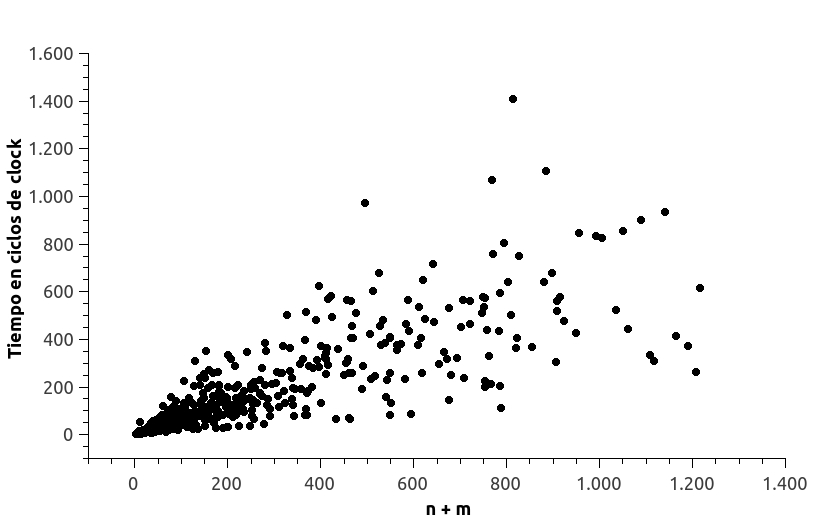
\includegraphics[width=\textwidth]{imagenes/ejer4-grafB1-1.jpg}
                \caption{Tiempos sin procesar}
        \end{subfigure}%
        ~ %add desired spacing between images, e. g. ~, \quad, \qquad, \hfill etc.
          %(or a blank line to force the subfigure onto a new line)
        \begin{subfigure}[b]{0.5\textwidth}
                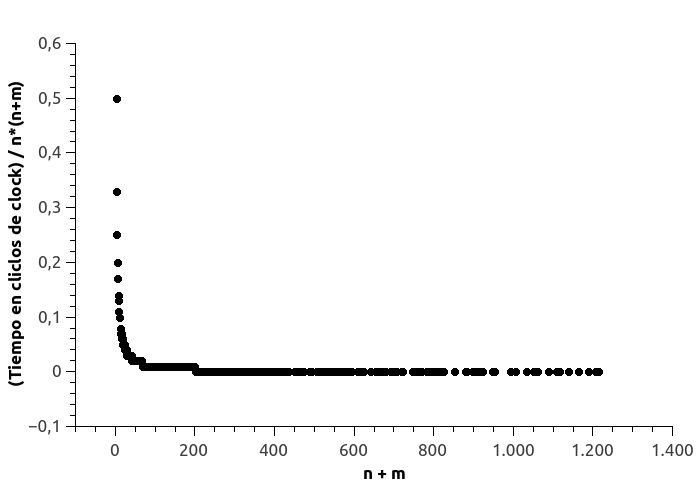
\includegraphics[width=\textwidth]{imagenes/ejer4-grafB1-2.jpg}
                \caption{figura (a) / n*(n+m)}
        \end{subfigure}

\end{figure}

\item \textbf{Tipo G1: Goloso-Primer Criterio de Vecindad}

\begin{figure}[H]
        \centering
        \begin{subfigure}[b]{0.5\textwidth}
                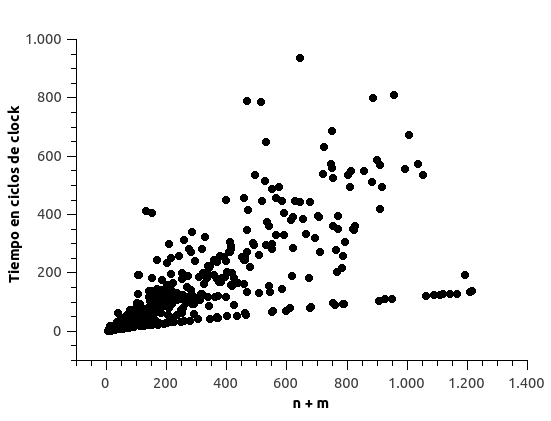
\includegraphics[width=\textwidth]{imagenes/ejer4-grafG1-1.jpg}
                \caption{Tiempos sin procesar}
        \end{subfigure}%
        ~ %add desired spacing between images, e. g. ~, \quad, \qquad, \hfill etc.
          %(or a blank line to force the subfigure onto a new line)
        \begin{subfigure}[b]{0.5\textwidth}
                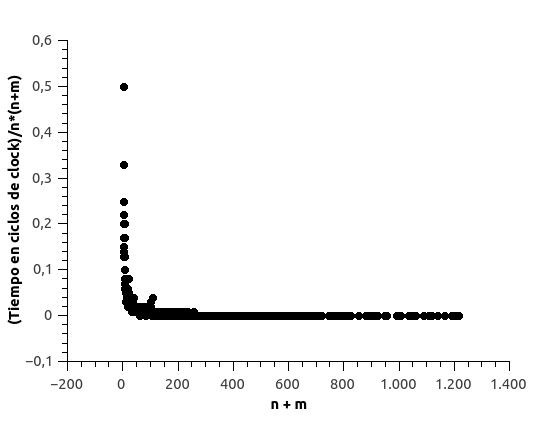
\includegraphics[width=\textwidth]{imagenes/ejer4-grafG1-2.jpg}
                \caption{figura (a) / n*(n+m)}
        \end{subfigure}

\end{figure}


\item \textbf{Tipo B2: BFS-Segundo Criterio de Vecindad}

\begin{figure}[H]
        \centering
        \begin{subfigure}[b]{0.5\textwidth}
                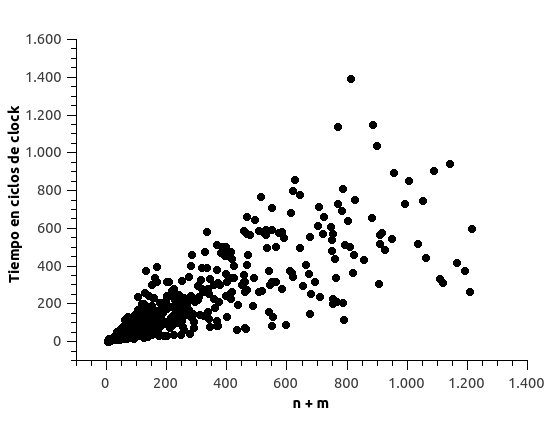
\includegraphics[width=\textwidth]{imagenes/ejer4-grafB2-1.jpg}
                \caption{Tiempos sin procesar}
        \end{subfigure}%
        ~ %add desired spacing between images, e. g. ~, \quad, \qquad, \hfill etc.
          %(or a blank line to force the subfigure onto a new line)
        \begin{subfigure}[b]{0.5\textwidth}
                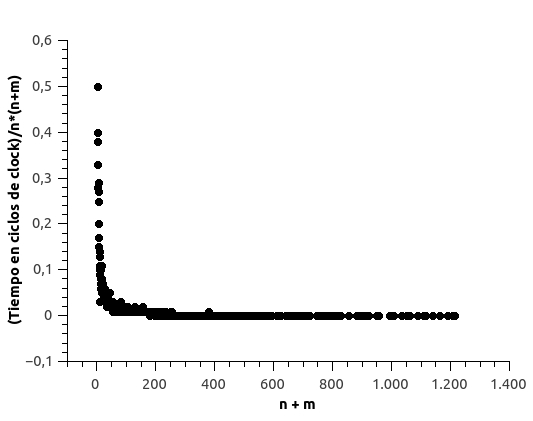
\includegraphics[width=\textwidth]{imagenes/ejer4-grafB2-2.jpg}
                \caption{figura (a) / n*(n+m)}
        \end{subfigure}

\end{figure}



\item \textbf{Tipo G2: Goloso-Segundo Criterio de Vecindad}

\begin{figure}[H]
        \centering
        \begin{subfigure}[b]{0.5\textwidth}
                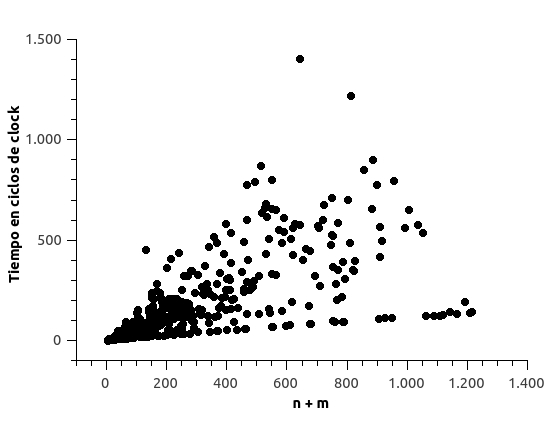
\includegraphics[width=\textwidth]{imagenes/ejer4-grafG2-1.jpg}
                \caption{Tiempos sin procesar}
        \end{subfigure}%
        ~ %add desired spacing between images, e. g. ~, \quad, \qquad, \hfill etc.
          %(or a blank line to force the subfigure onto a new line)
        \begin{subfigure}[b]{0.5\textwidth}
                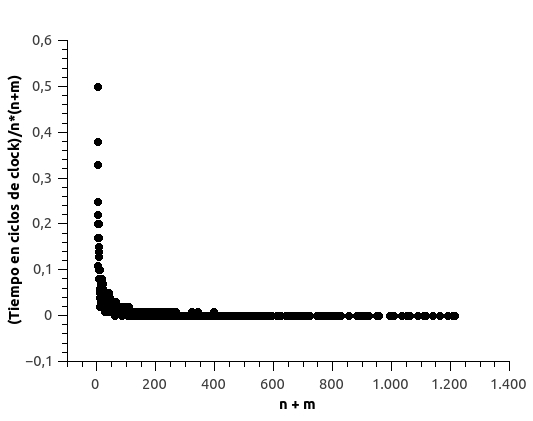
\includegraphics[width=\textwidth]{imagenes/ejer4-grafG2-2.jpg}
                \caption{figura (a) / n*(n+m)}
        \end{subfigure}

\end{figure}


\end{enumerate}

Como podemos ver de los 4 gráficos, al dividir los tiempos por $n*(n+m)$, tienden a un número constante mayor a cero. Entonces nuestro algoritmo tendría complejidad $\mathcal{O}(c*n*(n+m))$, donde $c$ es la constante a la cual converge el gráfico. Por lo tanto concluimos que la complejidad temporal experimental coincide con nuestra predicción de complejidad.


Por el lado de la calidad de las soluciones obtenidas con cada combinación, debemos comparar por un lado el uso del BFS modificado o de la heurística golosa como solución inicial y por el otro el uso del primer criterio de vecindad o el del segundo criterio de vecindad como método de mejora de la solución inicial:
\begin{itemize}
\item \textbf{BFS modificado vs Heurística golosa como solución inicial}. Para realizar la comparación, tomamos el tamaño de la solución final para cada instancia, usando primero el BFS modificado como solución inicial y luego la heurística golosa, para después restar al tamaño de la solución final del tipo B1/B2, el tamaño de la solución final del tipo G1/G2. :

\begin{figure}[H]
        \centering
        \begin{subfigure}[b]{0.5\textwidth}
                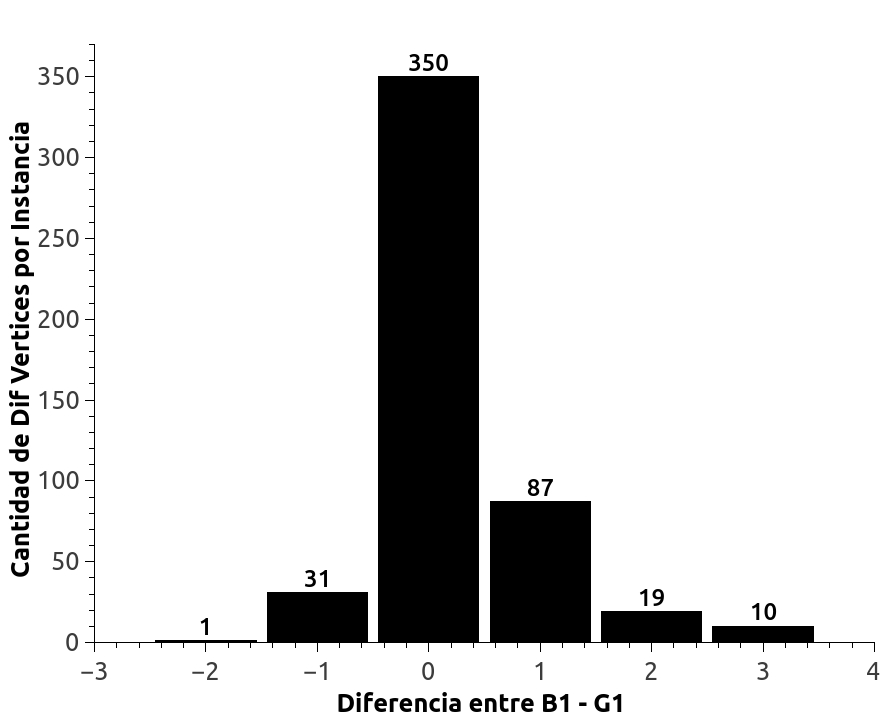
\includegraphics[width=\textwidth]{imagenes/ejer4-B1vsG1.jpg}
                \caption{Usando el Primer Criterio de Vecindad}
        \end{subfigure}%
        ~ %add desired spacing between images, e. g. ~, \quad, \qquad, \hfill etc.
          %(or a blank line to force the subfigure onto a new line)
        \begin{subfigure}[b]{0.5\textwidth}
                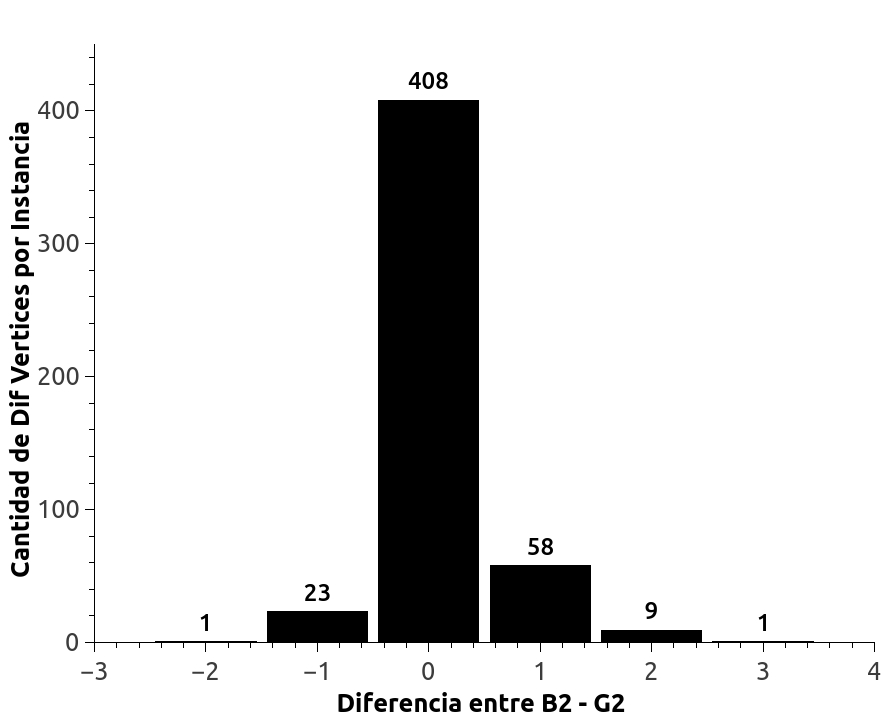
\includegraphics[width=\textwidth]{imagenes/ejer4-B2vsG2.jpg}
                \caption{Usando el Segundo Criterio de Vecindad}
        \end{subfigure}

\end{figure}

\end{itemize}

En ambos casos, se aprecia una paridad entre ambos soluciones, sin embargo hay una leve tendencia hacia la heurística golosa como mejor procedimiento para construir la solución inicial.

\begin{itemize}
	\item \textbf{Criterio de Vencindad}. El análisis comparado es el siguiente (utilizando la misma metodología que en el caso de BFS vs Golosa):

    \begin{figure}[H]
        \centering
        \begin{subfigure}[b]{0.5\textwidth}
                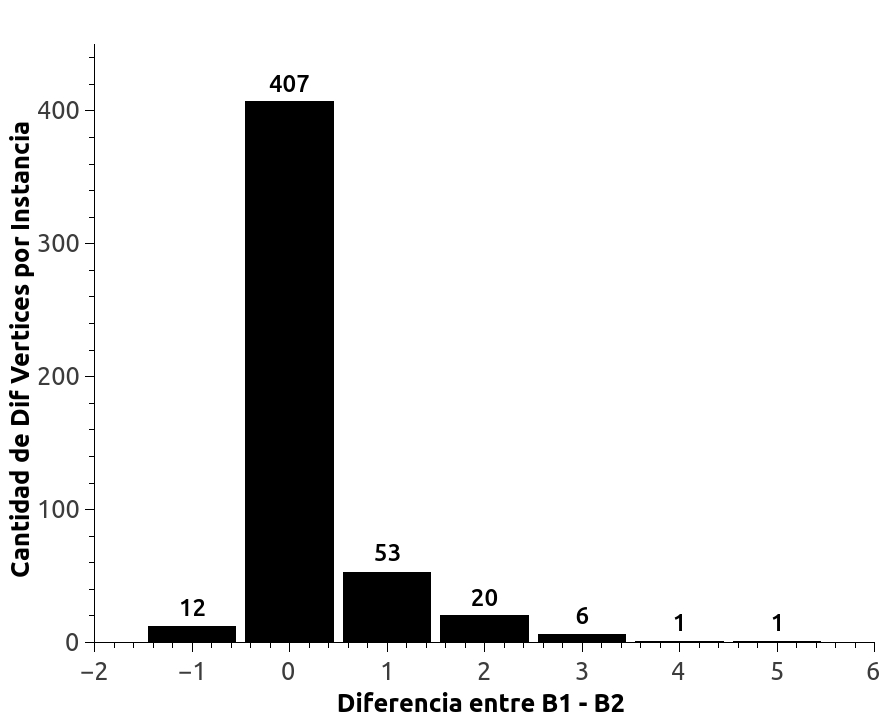
\includegraphics[width=\textwidth]{imagenes/ejer4-B1vsB2.jpg}
                \caption{Usando BFS como solucion incial}
        \end{subfigure}%
        ~ %add desired spacing between images, e. g. ~, \quad, \qquad, \hfill etc.
          %(or a blank line to force the subfigure onto a new line)
        \begin{subfigure}[b]{0.5\textwidth}
                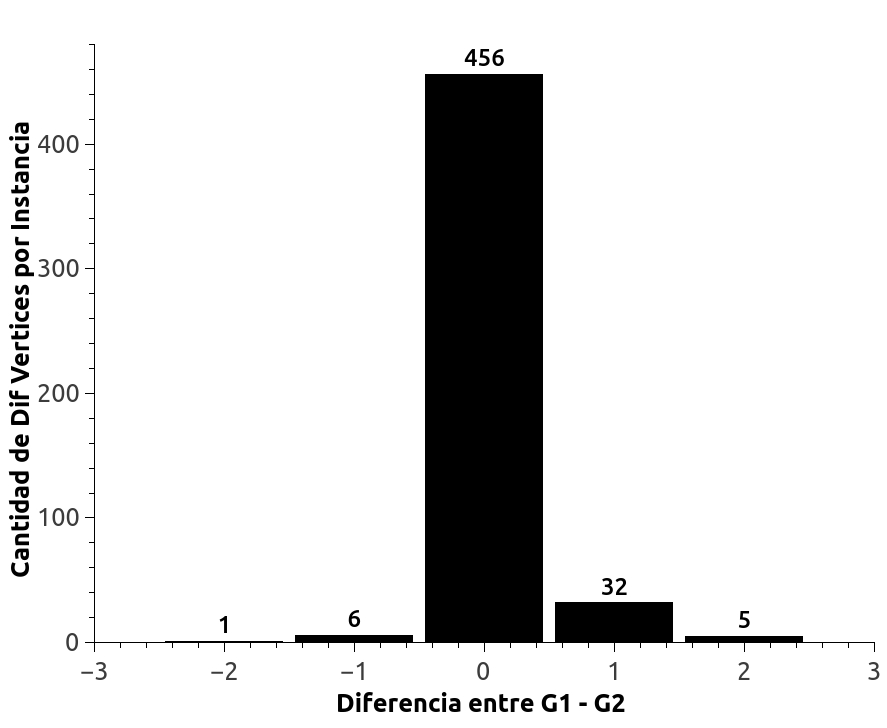
\includegraphics[width=\textwidth]{imagenes/ejer4-G1vsG2.jpg}
                \caption{Usando Goloso como solucion incial}
        \end{subfigure}

\end{figure}


\end{itemize}



Estos resultados nos inclinan a pensar que el segundo criterio de vecindad es el mejor criterio, lo cual es coherente con el hecho que el segundo criterio de vecindad es capaz de arreglar soluciones que el primer criterio de vecindad da como invalidas. Es decir, podríamos argumentar que como el primer criterio de vecindad es un caso particular del segundo criterio de vecindad (cuando no incluimos ningún vértice al subconjunto, mas allá del candidato) debería ser siempre mejor al primero. Sin embargo, la experimentación muestra casos donde el primer criterio es mejor, y eso se da en instancias donde arreglar una solución invalida nos inhibe de seguir explorando la solución original en búsqueda de un mejor caso. Por ejemplo:

\begin{itemize}

	\item Grafo de n = 9 y m = 13

\tikz[every node/.style={draw,circle}] {
	\node (1) at (0, 0)  { 1 };
	\node (2) at (4.5, 0)  { 2 };
	\node (3) at (2, -2)  { 3 };
	\node (4) at (2, 2)  { 4 };
	\node (5) at (7.5, -1.5)  { 5 };
	\node (6) at (1, -1)  { 6 };
	\node (7) at (3, 0)  { 7 };
	\node (8) at (2.5, -1)  { 8 };
	\node (9) at (4, -1)  { 9 };
	\draw (1) edge node[above,draw=none] {} (6);
	\draw (3) edge node[above,draw=none] {} (5);
	\draw (4) edge node[above,draw=none] {} (6);
	\draw (6) edge node[above,draw=none] {} (7);
	\draw (6) edge node[above,draw=none] {} (3);
	\draw (5) edge node[above,draw=none] {} (4);
	\draw (7) edge node[above,draw=none] {} (4);
	\draw (7) edge node[above,draw=none] {} (8);
	\draw (9) edge node[above,draw=none] {} (8);
	\draw (9) edge node[above,draw=none] {} (5);
	\draw (9) edge node[above,draw=none] {} (2);
	\draw (7) edge node[above,draw=none] {} (2);
	\draw (8) edge node[above,draw=none] {} (3);
}



\item \textbf{Solución Golosa}: como el mayor grado, 3, es compartido por varios vertices, empezamos por el menor numero de etiqueta, que es el 5, y asi sucesivamente.

\tikz[every node/.style={draw,circle}] {
	\node (1) at (0, 0)  { 1 };
	\node (2)[fill=blue!40, text=white] at (4.5, 0)  { 2 };
	\node (3) at (2, -2)  { 3 };
	\node (4) at (2, 2)  { 4 };
	\node (5)[fill=blue!40, text=white] at (7.5, -1.5)  { 5 };
	\node (6)[fill=blue!40, text=white] at (1, -1)  { 6 };
	\node (7) at (3, 0)  { 7 };
	\node (8)[fill=blue!40, text=white] at (2.5, -1)  { 8 };
	\node (9) at (4, -1)  { 9 };
	\draw (1) edge node[above,draw=none] {} (6);
	\draw (3) edge node[above,draw=none] {} (5);
	\draw (4) edge node[above,draw=none] {} (6);
	\draw (6) edge node[above,draw=none] {} (7);
	\draw (6) edge node[above,draw=none] {} (3);
	\draw (5) edge node[above,draw=none] {} (4);
	\draw (7) edge node[above,draw=none] {} (4);
	\draw (7) edge node[above,draw=none] {} (8);
	\draw (9) edge node[above,draw=none] {} (8);
	\draw (9) edge node[above,draw=none] {} (5);
	\draw (9) edge node[above,draw=none] {} (2);
	\draw (7) edge node[above,draw=none] {} (2);
	\draw (8) edge node[above,draw=none] {} (3);
}


\item \textbf{Solución aplicando el segundo criterio de vecindad a la solución golosa}: tenemos 4 candidatos que cumplen con el hecho de tener 2 o mas adyacentes incluidos: 3, 4, 7, 9.
\begin{enumerate}
	\item Vértice 3: incluimos el 3, quitamos el 5, 6 y 8, por lo tanto podemos incluir un vértice mas, que sera el 1. Sin embargo el 4 no es dominado por nadie, por lo cual no es una solución valida.
		\item Vértice 4: incluimos el 4, y quitamos el 5 y el 6. No podemos incluir ningún vértice mas, por lo tanto el 1 no es dominado por nadie, no es una solución valida.
		\item Vértice 7: incluimos el 7 y quitamos el 2, 6 y 8. Incluimos el 1, y nos queda una solución valida.
		\item Vértice 9: no es contemplado, ya que obtuvimos una solución mejor con el vértice 7. Solución que ya no es posible mejorar.
\end{enumerate}
\tikz[every node/.style={draw,circle}] {
	\node (1)[fill=blue!40, text=white] at (0, 0)  { 1 };
	\node (2) at (4.5, 0)  { 2 };
	\node (3) at (2, -2)  { 3 };
	\node (4) at (2, 2)  { 4 };
	\node (5)[fill=blue!40, text=white] at (7.5, -1.5)  { 5 };
	\node (6) at (1, -1)  { 6 };
	\node (7)[fill=blue!40, text=white] at (3, 0)  { 7 };
	\node (8) at (2.5, -1)  { 8 };
	\node (9) at (4, -1)  { 9 };
	\draw (1) edge node[above,draw=none] {} (6);
	\draw (3) edge node[above,draw=none] {} (5);
	\draw (4) edge node[above,draw=none] {} (6);
	\draw (6) edge node[above,draw=none] {} (7);
	\draw (6) edge node[above,draw=none] {} (3);
	\draw (5) edge node[above,draw=none] {} (4);
	\draw (7) edge node[above,draw=none] {} (4);
	\draw (7) edge node[above,draw=none] {} (8);
	\draw (9) edge node[above,draw=none] {} (8);
	\draw (9) edge node[above,draw=none] {} (5);
	\draw (9) edge node[above,draw=none] {} (2);
	\draw (7) edge node[above,draw=none] {} (2);
	\draw (8) edge node[above,draw=none] {} (3);
}


\item \textbf{Solución aplicando el primer criterio de vecindad a la solución golosa}: los candidatos son los mismos que en el segundo criterio, sin embargo al no poder incluir vértice mas allá del candidato, la solución probando con el vértice 7 es invalida, ya que el 1 no es dominado por nadie. Por lo tanto probamos con incluir el 9, y quitar el 2, 5 y 8. Al hacer esto nos queda una solución valida de menor cardinal que en la solución golosa original y que si hubiésemos utilizado el segundo criterio

\tikz[every node/.style={draw,circle}] {
	\node (1) at (0, 0)  { 1 };
	\node (2) at (4.5, 0)  { 2 };
	\node (3) at (2, -2)  { 3 };
	\node (4) at (2, 2)  { 4 };
	\node (5) at (7.5, -1.5)  { 5 };
	\node (6)[fill=blue!40, text=white] at (1, -1)  { 6 };
	\node (7) at (3, 0)  { 7 };
	\node (8) at (2.5, -1)  { 8 };
	\node (9)[fill=blue!40, text=white] at (4, -1)  { 9 };
	\draw (1) edge node[above,draw=none] {} (6);
	\draw (3) edge node[above,draw=none] {} (5);
	\draw (4) edge node[above,draw=none] {} (6);
	\draw (6) edge node[above,draw=none] {} (7);
	\draw (6) edge node[above,draw=none] {} (3);
	\draw (5) edge node[above,draw=none] {} (4);
	\draw (7) edge node[above,draw=none] {} (4);
	\draw (7) edge node[above,draw=none] {} (8);
	\draw (9) edge node[above,draw=none] {} (8);
	\draw (9) edge node[above,draw=none] {} (5);
	\draw (9) edge node[above,draw=none] {} (2);
	\draw (7) edge node[above,draw=none] {} (2);
	\draw (8) edge node[above,draw=none] {} (3);
}

\end{itemize}

Sin embargo estos tipos de instancias son muy particulares, por lo cual podemos afirmar que la \textbf{mejor combinación} para la \textbf{heurística de búsqueda local} planteada es aquella que toma como \textbf{solución inicial} la generada por la \textbf{heurística golosa} y luego es mejorada por el \textbf{segundo criterio de vecindad}.
